\section*{2. Theory}

\subsection*{Gate-level and Dataflow Modeling}
\begin{itemize}[leftmargin=*]
    \item \textbf{Gate-level modeling} describes a circuit by specifying its gates and how they are connected, using primitive gates such as \texttt{and}, \texttt{or} and \texttt{not}. Internal connections are declared as \texttt{wire}.
    \item \textbf{Dataflow modeling} describes the Boolean equations of combinational logic directly with continuous assignments using the keyword \texttt{assign}, without caring about the gate-level structure, e.g.\ \texttt{assign F = A \& B;}.
\end{itemize}

\subsection*{Operators in Verilog}
\begin{table}[H]
\centering
\small
\begin{tabular}{c l @{\hspace{2em}} c l}
\toprule
\multicolumn{2}{c}{\textbf{Bit-wise}} & \multicolumn{2}{c}{\textbf{Logical}} \\
\midrule
\verb|~|  & NOT  & \verb|!|  & logical NOT \\
\verb|&|  & AND  & \verb|&&| & logical AND \\
\verb+|+  & OR   & \verb+||+ & logical OR \\
\verb|^|  & XOR  & & \\
\verb|~^| or \verb|^~| & XNOR & & \\
\bottomrule
\end{tabular}
\captionof{table}{Bit-wise and logical operators}
\end{table}
Bit-wise operators act on each bit of the operands, while the operands of a logical operator are interpreted as false (all bits 0) or true (at least one bit 1), and the result is always 1 bit. For 1-bit signals the two kinds can be used interchangeably. Verilog also provides arithmetic operators (\verb|+ - * / %|) and relational operators (\verb|< <= > >= == !=|).

\subsection*{Exp-5a: Combinational Circuit}
\begin{figure}[H]
    \centering
    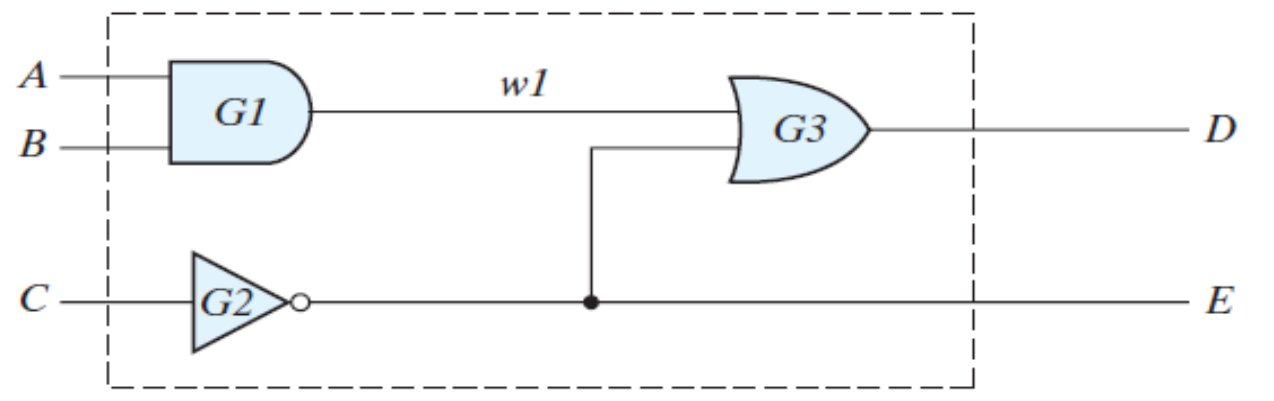
\includegraphics[width=0.6\textwidth]{pic/5a_circuit.png}
    \captionof{figure}{Logic circuit of Exp-5a}
    \label{fig:5a_circuit}
\end{figure}
The circuit has three inputs ($A$, $B$, $C$), so there are $2^3 = 8$ possible input combinations. Its outputs are
\[
    w_1 = A \cdot B, \qquad E = \overline{C}, \qquad D = w_1 + E = A \cdot B + \overline{C}.
\]

\subsection*{Exp-5b: Boolean Function}
\[
    F = (A \cdot B) \oplus (B \downarrow C), \qquad B \downarrow C = \overline{B + C} \ \text{(NOR)}
\]
With $w_1 = A \cdot B$ and $w_2 = \overline{B + C}$, the function becomes $F = w_1 \oplus w_2 = w_1 \overline{w_2} + \overline{w_1} w_2$.
